\documentclass[crop,tikz]{standalone}

\usepackage{tikz}

\begin{document}

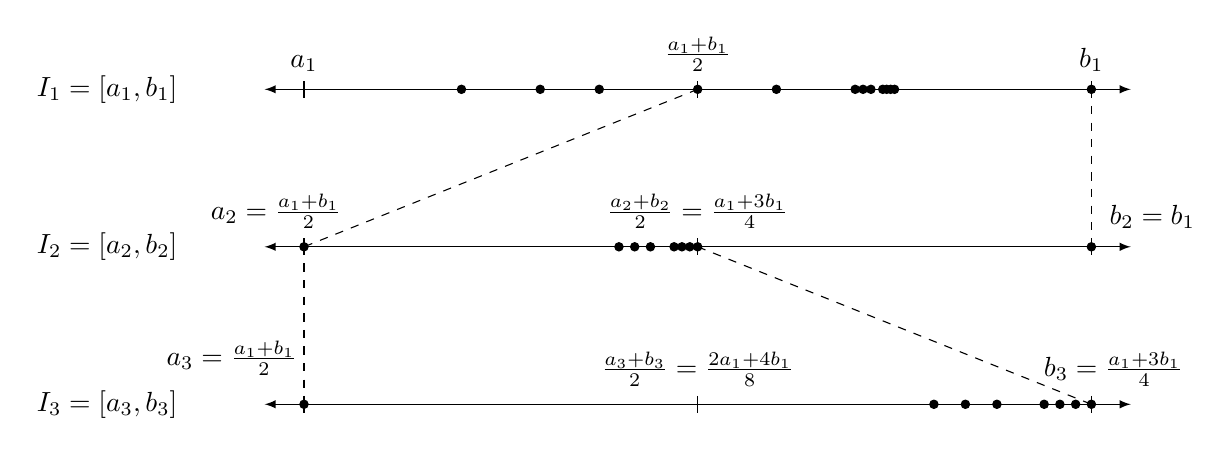
\begin{tikzpicture}

\node at (-7.5,0) {$I_1 = [a_1,b_1]$};
\draw[latex-latex] (-5.5,0) -- (5.5,0) ; %edit here for the axis
\foreach \x in {-5,0,5}
  \draw[shift={(\x,0)},color=black] (0pt,3pt) -- (0pt,-3pt);
\draw[shift={(-5,0)},color=black] (0pt,0pt) -- (0pt,-3pt) node[above,yshift=6] 
{$a_1$};
\draw[shift={(5,0)},color=black] (0pt,0pt) -- (0pt,-3pt) node[above,yshift=6] 
{$b_1$};
\draw[shift={(0,0)},color=black] (0pt,0pt) -- (0pt,-3pt) node[above,yshift=6] 
{$\frac{a_1+b_1}{2}$};
\foreach \x in {-3,-2,-1.25,1,0,2,2.1,2.2,2.35,2.4,2.45,2.5,5}
  \draw[shift={(\x,0)},color=black,fill] (0,0) circle (1.5pt);

\draw[dashed] (0,0) -- (-5,-2);
\draw[dashed] (5,0) -- (5,-2);

\begin{scope}[yshift=-2cm]
\node at (-7.5,0) {$I_2 = [a_2,b_2]$};
\draw[latex-latex] (-5.5,0) -- (5.5,0) ; %edit here for the axis
\foreach \x in {-5,0,5}
  \draw[shift={(\x,0)},color=black] (0pt,3pt) -- (0pt,-3pt);
\draw[shift={(-5,0)},color=black] (0pt,0pt) -- (0pt,-3pt) node[above,xshift=-10,yshift=6] 
{$a_2 = \frac{a_1+b_1}{2}$};
\draw[shift={(5,0)},color=black] (0pt,0pt) -- (0pt,-3pt) node[above,xshift=22,yshift=6] 
{$b_2=b_1$};
\draw[shift={(0,0)},color=black] (0pt,0pt) -- (0pt,-3pt) node[above,yshift=6] 
{$\frac{a_2+b_2}{2}=\frac{a_1+3 b_1}{4}$};
\foreach \x in {-5,-1,-0.8,-0.6,-0.3,-0.2,-0.1,0,5}
  \draw[shift={(\x,0)},color=black,fill] (0,0) circle (1.5pt);
\end{scope}

\draw[dashed] (-5,-2) -- (-5,-4);
\draw[dashed] (0,-2) -- (5,-4);

\begin{scope}[yshift=-4cm]
\node at (-7.5,0) {$I_3 = [a_3,b_3]$};
\draw[latex-latex] (-5.5,0) -- (5.5,0) ; %edit here for the axis
\foreach \x in {-5,0,5}
  \draw[shift={(\x,0)},color=black] (0pt,3pt) -- (0pt,-3pt);
\draw[shift={(-5,0)},color=black] (0pt,0pt) -- (0pt,-3pt) node[above,xshift=-26,yshift=10] 
{$a_3 = \frac{a_1+b_1}{2}$};
\draw[shift={(5,0)},color=black] (0pt,0pt) -- (0pt,-3pt) node[above,xshift=8,yshift=6] 
{$b_3 = \frac{a_1+3 b_1}{4}$};
\draw[shift={(0,0)},color=black] (0pt,0pt) -- (0pt,-3pt) node[above,yshift=6] 
{$\frac{a_3+b_3}{2}=\frac{2a_1+4 b_1}{8}$};
\foreach \x in {-5,3,3.4,3.8,4.4,4.6,4.8,5}
  \draw[shift={(\x,0)},color=black,fill] (0,0) circle (1.5pt);
\end{scope}

\end{tikzpicture}

\end{document}

\end{document}